\documentclass{article}
\usepackage[utf8]{inputenc}
\usepackage{graphicx} % Required for including images

\title{Eserciziario}
\author{Leonardo Ranaldi }
\date{January 2019}

\begin{document}

\maketitle

\iffalse
\section{Algebre di Boole e funzioni logiche}

\subsection{Esercizio}
Rappresentare le funzioni logiche F e G in termini delle variabili A, B e C, in
forma normale congiuntiva e disgiuntiva e poi con solo operazioni NOR:

\vskip 0.3cm
\begin{tabular}{|p{0.2\textwidth}|p{0.2\textwidth}|p{0.2\textwidth}|p{0.2\textwidth}|p{0.2\textwidth}|}
\hline
A        & B              & C      & F      & G     \\
\hline
0            & 0             & 0      & 1    & 0  \\
0            & 0             & 1      & 0   & 0   \\
0            & 1             & 0      & 0    & 0  \\
0            & 1             & 1      & 0   & 0  \\
1            & 0             & 0      & 0    & 0  \\
1            & 0             & 1      & 0    & 0  \\
1            & 1             & 0      & 0    & 1  \\
1            & 1             & 1      & 0   & 0   \\
\hline
\end{tabular}

\vskip 0.5cm
\textbf{Soluzione}
\vskip 0.5cm

\textbf{Forma normale disgiuntiva:}
\begin{itemize}
\item Per ogni riga tavola verità con valore 1:
\begin{itemize}
 \item Variabili con valore 0 in forma negata;
 \item Variabili con valore 1 in forma positiva
 \item Prodotto tra variabili
\end{itemize}
\item  Somma espressioni ottenute
\end{itemize}

\textbf{Forma normale congiuntiva:}
\begin{itemize}
\item Per ogni riga tavola verità con valore 0:
\begin{itemize}
\item Variabili con valore 0 in forma positiva;
\item Variabili con valore 1 in forma negata;
\item  Somma tra variabili;
\end{itemize}
\item Prodotto espressioni ottenute.
\end{itemize}

\textbf{Forma normale disgiuntiva:}
\[ F = (\overline{ABC})+ ABC \]
\[ G = AB\overline{C} \]

\textbf{Forma normale congiuntiva:}
\[  \]

\fi


\section{Modello di multiprogrammazione}
\subsection{Esercizio}
In un computer con 1 GB di memoria, il sistema operativo occupa 512 MB e i processi occupano mediamente 128 MB, se l’attesa media dell’I/O è del 80\%, qual è l’utilizzo della CPU? Aggiungendo 512 MB di RAM quanto sarà il nuovo utilizzo della CPU?
\vskip 0.5cm
\textbf{Soluzione}\\
\begin{itemize}
\item Il tempo di attesa del 80\% è riferito all'attesa di completamento di operazioni di I/O.
\item Se abbiamo n processi in memoria e il tempo di attesa medio è p, allora la probabilità che tutti i processi siano in attesa (e quindi la CPU sia intattiva) è $p^n$.
\item L'utilizzo della CPU è, dunque, $1- p^n$.
\item Il numero n di processi è ottenibile dividendo la dimensione di RAM libera per lo spazio occupato naturalmente da un solo processo.
\item  p = 80\% 
\item  n = (1GB – 512 MB) / 128 MB = 512/128 = 4 
\item  Utilizzo CPU = $1- p^n$ = $1 - 0.8^4$ = 0.59 
\item  p = 80\% 
\item  Nuova RAM: 512MB 
\item  n = (1GB – 512 MB+512 MB) / 128 MB = 1024/128 = 8 
\item  Utilizzo CPU = $1- p^n$ = $1 – 0.8^8$ = 0.8322 
\end{itemize}

\subsection{Esercizio}

In un computer con 1 GB di memoria, il sistema operativo occupa 512 MB e i processi occupano mediamente 64 MB, se l’attesa media dell’I/O è del 60\%, qual è l’utilizzo della CPU? Aggiungendo 256 MB di RAM, quale sarà il nuovo utilizzo della CPU? 

\vskip 0.5cm
\textbf{Soluzione}\\

\begin{itemize}
\item Il tempo di attesa del 60\% è riferito all'attesa di completamento di operazioni di I/O.
\item Se abbiamo n processi in memoria e il tempo di attesa medio è p, allora la probabilità che tutti i processi siano in attesa (e quindi la CPU sia intattiva) è $p^n$.
\item L'utilizzo della CPU è, dunque, $1- p^n$.
\item Il numero n di processi è ottenibile dividendo la dimensione di RAM libera per lo spazio occupato naturalmente da un solo processo.
\item p = 60\% 
\item n = (1GB – 512 MB) / 64 MB = 512/64 = 8 
\item Utilizzo CPU = 1- $p^n$ = $1 - 0.6^8$ = 0.983 
\item p = 60\% 
\item Nuova RAM: 256MB 
\item n = (1GB – 512 MB+256) / 64 MB = 768/64 = 12 
\item Utilizzo CPU = 1- $p^n$ = $1 - 0.6^{12}$ = 0.997 
\end{itemize}


\subsection{Esercizio}

In un computer con 1 GB di memoria, il sistema operativo occupa 512 MB e i processi occupano mediamente 64 MB, se l’attesa media dell’I/O è del 65\%, qual è l’utilizzo della CPU? Aggiungendo 512 MB di RAM quanto sarà il nuovo utilizzo della CPU?
\vskip 0.5cm
\textbf{Soluzione}\\


\begin{itemize}
\item Il tempo di attesa del 65\% è riferito all'attesa di completamento di operazioni di I/O.
\item Se abbiamo n processi in memoria e il tempo di attesa medio è p, allora la probabilità che tutti i processi siano in attesa (e quindi la CPU sia intattiva) è $p^n$.
\item  L'utilizzo della CPU è, dunque, $1- p^n$.
\item  Il numero n di processi è ottenibile dividendo la dimensione di RAM libera per lo spazio occupato naturalmente da un solo processo.
\item  p = 65\% 
\item  n = (1GB – 512 MB) / 64 MB = 512/64 = 8 
\item  Utilizzo CPU = $1- p^n$ = $1 - 0.65^8$ = 0.968 
\item  p = 65\% 
\item  Nuova RAM: 512MB 
\item  n = (1GB – 512 MB+512 MB) / 64 MB = 1024/64 = 16 
\item  Utilizzo CPU = 1- $p^n$ = $1 – 0.65^{16}$ = 0.998 
\end{itemize}


\section{Soft real-time con eventi periodici}
\subsection{Esercizio}

Supponendo di dover valutare la fattibilità di un sistema soft real-time con eventi periodici $P_{0}=500 \mu s$, $P_{1}=300 \mu s$, $P_{2}=15 ms$, $P_{3} = 800 ms$.\\
Con rispettivi tempi di elaborazione $C_{0}=100 \mu s$, $C_{1}=100 \mu s$,
$C_{2}=3ms$, $C_{3}=200 ms$.\\
Il sistema è sostenibile? Se si aggiunge un nuovo evento periodico $P_4=100ms$, con $C_4= 2ms$. Il sistema rimane sostenibile? Perché?\\

\vskip 0.5cm
\textbf{Soluzione}\\

Deadline: tempo entro il quale le operazioni devono necessariamente
essere completate.\\
- Sistemi non obbligatoriamente veloci ma piuttosto affidabili.\\
- Eventi periodici: eseguiti a ciclo continuo con cadenza ben definita.\\
- Eventi periodici hanno:

\begin{itemize}
\item Periodo: tempo entro il quale l’evento deve essere ripetuto (Pi)
\item Tempo d’esecuzione (Ci)
\item Sistema Real Time sostenibile (con m eventi periodici): vale \[\sum_{i=1}^m \frac{C_i}{P_i} \le 1\]

\end{itemize}

Procediamo con la sostituzione dei valori all’interno della formula:
 \[ \frac{C_0}{P_0}+\frac{C_1}{P_1}+\frac{C_2}{P_2}+\frac{C_3}{P_3} \le 1\]
 Sostituendo in modo opportuno si ottiene:
 \[ \frac{100}{500}+\frac{100}{300}+\frac{3}{15}+\frac{200}{800} = \frac{59}{60} \le 1\]

(Riferimento testo: Moderni sistemi operativi, paragrafo 2.5.4. Schedulazione nei sistemi
real time, pag 135 e successive)\\

Massimo tempo di esecuzione per il nuovo processo $P_{4}$.
 \[ \frac{C_0}{P_0}+\frac{C_1}{P_1}+\frac{C_2}{P_2}+\frac{C_3}{P_3}+\frac{C_4}{P_4} \le 1\]
Dato  $P_{4}$ e  $C_{4}$ sostituire nuovamente i valori e verificare il risultato.
 \[ \frac{100}{500}+\frac{100}{300}+\frac{3}{15}+\frac{200}{800}+\frac{2}{4} = \frac{89}{60} \le 1\]
Ma attenzione perchè:
 \[  \frac{89}{60} \not\le 1\]
Si può concludere quindi che il sistema non rimane sostenibile.

\vskip 1.5cm

\subsection{Esercizio}

Supponendo di dover valutare la fattibilità di un sistema soft real-time con eventi periodici $P_ {0}=300 \mu s$, $P_{1}=900 \mu s$, $P_{2}=45 ms$, $P_{3} = 150 ms$.\\
Con rispettivi tempi di elaborazione $C_{0}=25 \mu s$, $C_{1}=300 \mu s$,
$C_{2}=9ms$, $C_{3}=50 ms$.\\
Il sistema è sostenibile? Se si aggiunge un nuovo evento periodico $P_{4}=110ms$, quanto è il tempo massimo di elaborazione affinché il sistema rimanga sostenibile?



\vskip 0.5cm
\textbf{Soluzione}\\

Deadline: tempo entro il quale le operazioni devono necessariamente
essere completate.\\
- Sistemi non obbligatoriamente veloci ma piuttosto affidabili.\\
- Eventi periodici: eseguiti a ciclo continuo con cadenza ben definita.\\
- Eventi periodici hanno:

\begin{itemize}
\item Periodo: tempo entro il quale l’evento deve essere ripetuto (Pi)
\item Tempo d’esecuzione (Ci)
\item Sistema Real Time sostenibile (con m eventi periodici): vale \[\sum_{i=1}^m \frac{C_i}{P_i} \le 1\]

\end{itemize}

Procediamo con la sostituzione dei valori all’interno della formula:
 \[ \frac{C_0}{P_0}+\frac{C_1}{P_1}+\frac{C_2}{P_2}+\frac{C_3}{P_3} \le 1\]
 Sostituendo in modo opportuno si ottiene:
 \[ \frac{25}{300}+\frac{300}{900}+\frac{9}{45}+\frac{50}{150} = \frac{57}{60} \le 1\]

(Riferimento testo: Moderni sistemi operativi, paragrafo 2.5.4. Schedulazione nei sistemi
real time, pag 135 e successive)\\

Massimo tempo di esecuzione per il nuovo processo $P_{4}$.
 \[ \frac{C_0}{P_0}+\frac{C_1}{P_1}+\frac{C_2}{P_2}+\frac{C_3}{P_3}+\frac{C_4}{P_4} \le 1\]
Dato  $P_{4}$ risolvere la disequazione precedente per trovare il valore di  $C_{4}$.
 \[  \frac{57}{60}+\frac{C_4}{100} \le 1\]
 \[  \frac{C_4}{100} \le 1 - \frac{57}{60}\]
 \[  C_4 \le  \frac{3}{60}  110\]
  \[  C_4 \le  5.5\]

Massimo tempo di esecuzione: 5.5ms\\

\vskip 1.5cm

\subsection{Esercizio3}

Supponendo di dover valutare la fattibilità di un sistema soft real-time con eventi periodici $P_{0}=500 \mu s$, $P_{1}=300 \mu s$, $P_{2}=15 ms$, $P_{3} = 500 ms$.\\
Con rispettivi tempi di elaborazione $C_{0}=50 \mu s$, $C_{1}=50 \mu s$,
$C_{2}=3ms$, $C_{3}=100 ms$.\\
Il sistema è sostenibile? Se si aggiunge un nuovo evento periodico $P_4=100ms$, con $C_4= 2ms$. Il sistema rimane sostenibile? Perché?\\

\vskip 0.5cm
\textbf{Soluzione}\\

Deadline: tempo entro il quale le operazioni devono necessariamente
essere completate.\\
- Sistemi non obbligatoriamente veloci ma piuttosto affidabili.\\
- Eventi periodici: eseguiti a ciclo continuo con cadenza ben definita.\\
- Eventi periodici hanno:

\begin{itemize}
\item Periodo: tempo entro il quale l’evento deve essere ripetuto (Pi)
\item Tempo d’esecuzione (Ci)
\item Sistema Real Time sostenibile (con m eventi periodici): vale \[\sum_{i=1}^m \frac{C_i}{P_i} \le 1\]

\end{itemize}

Procediamo con la sostituzione dei valori all’interno della formula:
 \[ \frac{C_0}{P_0}+\frac{C_1}{P_1}+\frac{C_2}{P_2}+\frac{C_3}{P_3} \le 1\]
 Sostituendo in modo opportuno si ottiene:
 \[ \frac{50}{500}+\frac{50}{300}+\frac{3}{15}+\frac{100}{500} = \frac{20}{30} \le 1\]

(Riferimento testo: Moderni sistemi operativi, paragrafo 2.5.4. Schedulazione nei sistemi
real time, pag 135 e successive)\\

Massimo tempo di esecuzione per il nuovo processo $P_{4}$.
 \[ \frac{C_0}{P_0}+\frac{C_1}{P_1}+\frac{C_2}{P_2}+\frac{C_3}{P_3}+\frac{C_4}{P_4} \le 1\]
Dato  $P_{4}$ e  $C_{4}$ sostituire nuovamente i valori e verificare il risultato.
 \[ \frac{50}{500}+\frac{50}{300}+\frac{3}{15}+\frac{100}{500}+\frac{2}{4} = \frac{45}{30} \le 1\]
Ma attenzione perchè:
 \[  \frac{45}{30} \not\le 1\]
Si può concludere quindi che il sistema non rimane sostenibile.



\section{Scheduling nei sistemi batch}
\subsection{Esercizio}

Supponendo di utilizzare l’algoritmo shortest job first per
lo scheduling in un sistema batch, se arrivano 4 job (in ordine A, B,
C e D) con i seguenti tempi di esecuzione A=8, B=4, C=2 e D=4 quali
sono i tempi di turnaround e quale il tempo medio?

\vskip 0.5cm
\textbf{Soluzione}\\
\begin{itemize}
\item  Shortest job firs: Viene eseguito il job minore per primo.
\item  Tempo turnaround: tempo che intercorre dal momento in cui un processo entra in coda per essere eseguito fino al termine della sua esecuzione.
\item Tempo di attesa: tempo che un processo trascorre in coda prima di essere eseguito.
\item  \textbf{TA}  (Time of arrival)  tempo assoluto di ingresso in coda di un processo.
\item  \textbf{TE}  (Time of execution) tempo necessario per l’esecuzione di un processo.
\end{itemize}
Tabella con TA e TE di ogni processo dell’esercizio.

\vskip 0.3cm
\begin{tabular}{|p{0.2\textwidth}|p{0.2\textwidth}|p{0.2\textwidth}|}
\hline
Processo        & TA              & TE      \\
\hline
A            & 0             & 8      \\
B            & 0             & 4      \\
C            & 0             & 2      \\
D            & 0             & 4      \\
\hline
\end{tabular}



%\begin{tabular}{|p{0.2\textwidth}|p{0.1\textwidth}p{0.2\textwidth}|p{0.3\textwidth}|}
%\hline
%Processo        & TA        &       & TE      \\
%\hline
%nero            & 0     & zero          &       \\
%marrone         & 1     & uno           &       \\
%rosso           & 2     & due           &       \\
%\hline
%\end{tabular}

\begin{itemize}
\item  Strategia SJF: ordine C-B-D-A.
\item  TS = Tempo assoluto di inizio di esecuzione di ogni processo.
\item  TF = tempo assoluto di fine dell’esecuzione di un processo.
\end{itemize}


\vskip 0.3cm
\begin{tabular}{|p{0.2\textwidth}|p{0.13\textwidth}|p{0.13\textwidth}|p{0.13\textwidth}|p{0.13\textwidth}|}
\hline
Processo        & TA              & TE      & TS      & TF      \\
\hline
A            & 0             & 8      & 10      & 18 \\
B            & 0             & 4      & 2      & 6      \\
C            & 0             & 2      & 0      & 2      \\
D            & 0             & 4      & 6      & 10      \\
\hline
\end{tabular}

\begin{itemize}
\item  TT = Tempo Turnaround = TF-TA
\item  TW = Tempo di attesa = TS-TA
\end{itemize}


\vskip 0.3cm
\begin{tabular}{|p{0.2\textwidth}|p{0.11\textwidth}|p{0.11\textwidth}|p{0.11\textwidth}|p{0.11\textwidth}|p{0.11\textwidth}|p{0.11\textwidth}|}
\hline
Processo        & TA              & TE      & TS      & TF     & TW      & TT       \\
\hline
A            & 0             & 8      &10      &18       & 10    &18  \\
B            & 0             & 4      &2      &6        & 2    &6  \\
C            & 0             & 2      &0      &2        & 0    &2  \\
D            & 0             & 4      &6      &10       & 6    &10 \\
\hline
\end{tabular}

\begin{itemize}
\item Tempo medio (entambi i casi): somma tempi e divisione per numero
processi.
\end{itemize}

\[TW(medio) = \frac{10+2+0+6}{4} = 4,5 \]
\[TT(medio) = \frac{18+6+2+10}{4} = 9 \]





\subsection{Esercizio}
Supponendo di utilizzare l’algoritmo first-come first-served per lo scheduling in un
sistema batch, se arrivano 4 job (in ordine A, poi B dopo 2ms, C dopo 4ms e D dopo 5ms)
con i seguenti tempi di esecuzione A=8, B=4, C=2 e D=4 quali sono i tempi di turnaround?
Qual è il tempo medio di turnaround e di attesa?
\vskip 0.5cm
\textbf{Soluzione}\\
\begin{itemize}
\item  First come – First served: Ordine in cui chi arriva prima viene eseguito per primo.
\item  Tempo turnaround: tempo che intercorre dal momento in cui un processo entra in coda per essere eseguito fino al termine della sua esecuzione.
\item Tempo di attesa: tempo che un processo trascorre in coda prima di essere eseguito.
\item  \textbf{TA}  (Time of arrival)  tempo assoluto di ingresso in coda di un processo.
\item  \textbf{TE}  (Time of execution) tempo necessario per l’esecuzione di un processo.
\end{itemize}
Tabella con TA e TE di ogni processo dell’esercizio.

\vskip 0.3cm
\begin{tabular}{|p{0.2\textwidth}|p{0.2\textwidth}|p{0.2\textwidth}|}
\hline
Processo        & TA              & TE      \\
\hline
A            & 0             & 8      \\
B            & 2             & 4      \\
C            & 4             & 2      \\
D            & 5             & 4      \\
\hline
\end{tabular}

\begin{itemize}
\item  Strategia FCFS (FIFO): ordine A-B-C-D.
\item  TS = Tempo assoluto di inizio di esecuzione di ogni processo.
\item  TF = tempo assoluto di fine dell’esecuzione di un processo.
\end{itemize}
\vskip 0.3cm
\begin{tabular}{|p{0.2\textwidth}|p{0.13\textwidth}|p{0.13\textwidth}|p{0.13\textwidth}|p{0.13\textwidth}|}
\hline
Processo        & TA              & TE      & TS      & TF      \\
\hline
A            & 0             & 8      & 0      & 8      \\
B            & 2             & 4      & 8      & 12      \\
C            & 4             & 2      & 12      & 14      \\
D            & 5             & 4      & 14      & 18      \\
\hline
\end{tabular}

\begin{itemize}
\item  TT = Tempo Turnaround = TF-TA
\item  TW = Tempo di attesa = TS-TA
\end{itemize}

\vskip 0.3cm
\begin{tabular}{|p{0.2\textwidth}|p{0.11\textwidth}|p{0.11\textwidth}|p{0.11\textwidth}|p{0.11\textwidth}|p{0.11\textwidth}|p{0.11\textwidth}|}
\hline
Processo        & TA              & TE      & TS      & TF     & TW      & TT       \\
\hline
A            & 0             & 8      & 0      & 8       & 0  & 8 \\
B            & 2             & 4      & 8      & 12       & 6  & 10 \\
C            & 4             & 2      & 12      & 14      & 8  & 10 \\
D            & 5             & 4      & 14      & 18       & 9  & 13 \\
\hline
\end{tabular}
\begin{itemize}
\item Tempo medio (entambi i casi): somma tempi e divisione per numero
processi.
\end{itemize}

\[TW(medio) = \frac{0+6+8+9}{4} = 5.75 \]
\[TT(medio) = \frac{8+10+10+13}{4} = 10.25 \]

\subsection{Esercizio}
Supponendo di utilizzare l’algoritmo round–robin per lo scheduling in un sistema interattivo, se la coda è fatta dai processi A-B-C-D-E, nel caso in cui il quanto sia di 100 ms e il un tempo di cambio di contesto di 1 ms, quanto tempo sarà necessario prima che E venga eseguito? Qual è il rapporto tra cambio di contesto e tempo di esecuzione?
Come cambiano I tempi analizzati nel caso in cui il quanto sia, invece, di 4 ms?
Quale delle due soluzioni sembra più favorevole?
\vskip 0.5cm
\textbf{Soluzione}
\vskip 0.5cm

\textbf{Round- robin:}\\
Ad ogni processo viene assegnato un quanto di tempo in cui può andare in esecuzione, i processi vengono assegnati alla CPU tramite una coda circolare.\\
Se ha una richiesta bloccante o è terminato prima dello scadere del quanto, la CPU viene immediatamente assegnata al processo successivo.\\
Al termine di un quanto di tempo, viene cambiato l’assegnamento alla CPU, e deve intercorrere un certo tempo, il tempo di cambio di contesto prima che il nuovo processo possa iniziare la propria esecuzione.

\begin{itemize}

\item \textbf{E}: devono essere eseguiti per il loro quanto A, B, C e D e i ripettivi cambi di contesto. Quindi E deve aspettare, per la sua prima parte di esecuzione:
\[100 + 1 + 100 +1 + 100 + 1 + 100 + 1 =404 ms\]
(quasi mezzo secondo)
\item \textbf{Il rapporto è molto semplice:} 1ms/100ms = 0.01, (l’1\%)

\vskip 0.5cm

\item \textbf{Secondo caso:} \[4 + 1 + 4 + 1 + 4 + 1 + 4 + 1 =20 ms\]
\item  \textbf{Il rapporto è:} 1ms/4ms = 0.25, (il 25\%)

\vskip 0.5cm

\item \textbf{Confronto:} pro prima soluzione:
\begin{enumerate}
    \item Tempo cambio di contensto molto più piccolo di tempo esecuzione;
    \item Processi con lunghe CPU burst favoriti;
\end{enumerate}

\item  \textbf{Confronto:} contro prima soluzione:
\begin{enumerate}
    \item  Tempo attesa processi potenzialmente lungo (400 ms è un tempo considerevole);
    \item Se frequenti I/O burst, simile a seconda soluzione;
\end{enumerate}

\item  \textbf{Confronto:} pro seconda soluzione:
\begin{enumerate}
    \item  Processi hanno tempo di attesa basso, importante specialmente se forniti di iterfaccia utente;
\end{enumerate}
\item  \textbf{Confronto:} contro seconda soluzione:
\begin{enumerate}
    \item  Cambio contesto è rilevante: confrontabile con tempo esecuzione;
    \item  Sfavorisce processi con lunghe CPU burst;
\end{enumerate}
\end{itemize}




\section{Algoritmi di sostituzione delle pagine}
\subsection{Esercizio}

Supponendo di utilizzare l’algoritmo di sostituzione delle
pagine Not Recently Used (NRU), se la situazione è la seguente:
Classe 1 = pag.2, Classe 0 = pag.3, Classe 3 = pag.4, Classe 2 = pag.5
Specificare quale pagina verrà posta su disco se accade un page fault
spiegando le ragioni.
\vskip 0.5cm
\textbf{Soluzione}\\
La maggior parte dei computer con memoria virtuale prevede 2 bit per la raccolta di informazioni sull'utilizzo delle pagine:
\begin{itemize}
\item  il bit R: indica che la pagina è stata referenziata (letta o scritta)
\item  il bit M: indica che la pagina è stata modificata (scritta)
\end{itemize}

Algoritmo NRU (Not Recently Used)

\begin{enumerate}
\item  Inizialmente i bit R e M vengono impostati a 0 dal SO
\item  Periodicamente (ad esempio ad ogni interrupt del clock), il bit R viene azzerato per distinguere le pagine non referenziate recentemente dalle altre.
\end{enumerate}
Quando avviene un page fault, il SO controlla tutte le pagine e le divide in quattro classi in base al valore corrente dei bit R e M.

\vskip 0.5cm

 \begin{tabular}{|p{0.2\textwidth}|p{0.1\textwidth}|p{0.1\textwidth}|p{0.6\textwidth}|}
\hline
Classe         & R        & M          & Osservazioni \\
\hline
1            & 0     & 0               & classe più conveniente da swappare  \\
2            & 0     & 1                 &  \\
3            & 1     & 0                 & \\
4            & 1     & 1                &   classe meno conveniente da swappare \\
\hline
\end{tabular}

\vskip 0.5cm
 L'algoritmo NRU rimuove una pagina qualsiasi (a caso) dalla classe di numero inferiore che sia non vuota.\\
 
 \vskip 0.5cm
 
 \textbf{ Caratteristiche di NRU}: è facile da implementare ed  ha prestazioni che, anche se non ottimali, sono spesso adeguate.\\

 \vskip 0.5cm
 Dopo una breve introduzione possiamo dire che in caso di page fault la pag.3 verrà scartat poichè è a livello più basso di tutti mentre la pagina 4 verrà posta sul disco poichè appartiene alla classe maggiore.


\subsection{Esercizio}

Nell’ambito del rimpiazzamento delle pagine, supponendo di usare l’algoritmo not recently used (NRU), e seguendo la tabella delle pagine in figura, nel caso in cui avvenga
un page fault, quale sarà la pagina che verrà posta su disco? Perché?
Se invece considerassimo la tabella come una lista ordinata (nell’ordine A,...,G), cosa succederebbe per l’algoritmo second chance? Quale pagina sarebbe rimpiazzata?

\vskip 0.5cm


\begin{tabular}{|p{0.2\textwidth}|p{0.2\textwidth}|p{0.2\textwidth}|}
\hline
Pagina         & R        & M            \\
\hline
A            & 1     & 0                 \\
B            & 1     & 1                  \\
C            & 1     & 0                  \\
D            & 0     & 1                    \\
E            & 0     & 0                   \\
F            & 1     & 1                   \\
G            & 1     & 0                   \\
\hline
\end{tabular}

\vskip 1.5cm

\textbf{Soluzione}\\

\begin{itemize}
\item Bit R: posto a 1 ogni qual volta pagina sia riferita (cioè scritta o letta).
\item Bit M: posto a 1 ogni qual volta pagina sia modificata.
\item  Reset a 0 da software per entrambi i bit.
\item  Priorità :
\end{itemize}

\vskip 0.5cm

 \begin{tabular}{|p{0.2\textwidth}|p{0.1\textwidth}|p{0.1\textwidth}|p{0.6\textwidth}|}
\hline
Classe         & R        & M          & Osservazioni \\
\hline
1            & 0     & 0               & classe più conveniente da swappare  \\
2            & 0     & 1                 &  \\
3            & 1     & 0                 & \\
4            & 1     & 1                &   classe meno conveniente da swappare \\
\hline
\end{tabular}


\vskip 0.5cm


\textit{ALGORITMO SECOND CHANCE}
 Pagine in lista per ordine di ingresso.\\
 Bit M non considerato.\\
 \vskip 0.3cm
 \textbf{Algoritmo:}
\begin{itemize}
\item  Scorrere la lista
\item  Se R = 1, porre R=0, reinserire pagina in fondo a lista;
\item  Se R=0, effettuare swap della pagina corrispondente.
\item  Soluzione algoritmo LRU:
\item  Una sola pagina appartiene alla Classe 0, con massima priorità di swap.
\item  La pagina è E (M=0, R=0).
\item  Soluzione algoritmo second chance:
\item  A ha R=1: reset a 0 e spostamento in fondo alla lista,
\item  B ha R=1: reset a 0 e spostamento in fondo alla lista,
\item  C ha R=1: reset a 0 e spostamento in fondo alla lista,
\item  D ha R=0: swap su disco
\end{itemize}
Situazione finale in figura.

\vskip 0.3cm

\begin{tabular}{|p{0.2\textwidth}|p{0.2\textwidth}|}
\hline
Pagina         & R                \\
\hline
E                 & 0                 \\
F                 & 1                  \\
G                 & 1                  \\
A                 & 0                    \\
B                 & 0                   \\
C                 & 0                   \\
\hline
\end{tabular}


\iffalse
\newpage


%%%%%%%%%%%%%%%%%%%%%% DA TERMINARE %%%%%%%%%%%%%%%%%%%


\subsection{Esercizio}
 Supponendo di utilizzare l’algoritmo di sostituzione delle
pagine Aging con 6 frame e un contatore a 8 bit, se i valori di R
corrispondenti ai 6 frame [pag.0 pag.1…pag.5] dopo 5 clock sono
[000001, 010000, 110001, 001010, 110011]. Quale pagina verrà posta su
disco se accade un page fault? Perché?
\vskip 0.5cm
%\textbf{Soluzione}\\



%%%%%%%%%%%%%%%%%%%%%% DA TERMINARE %%%%%%%%%%%%%%%%%%%

\subsection{Esercizio}
Supponendo di disporre dei seguenti tempi di esecuzione $T_0, T_1, T_2$ e $T_3$ nell'algoritmo shortest process next con tecnica di aging, quale sarà la stima per $T_4$?	


\subsection{Esercizio}
Utilizzando l’algoritmo di paginazione Aging (con contatore a 8 bit), si
considerino le seguenti 4 pagine, con valore di bit R, rispettivamente, 1000. Ai
cicli successivi, i valori sono 0111, 0011, 1101, 1100, 0001, 1010 e 1110. Si
forniscano i valori dei 4 contatori dopo l’ultimo intervallo, specificando quale
pagina viene spostata su disco.
\vskip 0.5cm

%%%%%%%%%%%%%%%%%%%%%% DA TERMINARE %%%%%%%%%%%%%%%%%%%





\subsection{Esercizio}
Nella gestione delle locazioni libere della memoria, la
lista collegata contiene i seguenti elementi (formato: (Processo/Hole,
Posizione iniziale, lunghezza)):
(P0,0,5) $\to$ (H,5,3)$\to$ (P1,8,6)$\to$ (H,14,5)$\to$ (P2,19,4)$\to$ (H,23,4)$\to$ (P3,27,2)$\to$ (P4,29,1)$\to$ (H,30,6).\\
Se arriva il processo P che occupa 5 unità quale sarà la nuova
situazione della lista se l’algoritmo è il first fit? Scrivere la
nuova lista collegata a seguito dell’inserimento.
\vskip 0.5cm

\section{Algoritmi di scheduling delle richieste al disco}
\subsection{Esercizio}
1) Supponendo di utilizzare un disco con 40 cilindri e un
algoritmo di scheduling delle richieste first-come first-served
(FCFS), con posizione iniziale al cilindro 11 e che arrivino le
seguenti richieste sui cilindri 1, 36, 16, 34, 9 e 12. Quale sarà il
numero totale di spostamenti del braccio che alloggia la testina?

\fi


\section{Gestione della memoria, paginazione e gestione del disco}
\subsection{Esercizio}
 Nell’ambito della gestione della memoria con liste concatenate,
considerando una lista parzialmente piena di questo tipo (per ogni tripla, il primo elemento è un flag per capire se si tratta di un buco o un processo, il secondo è l’indirizzo di partenza e il terzo è la lunghezza dell’elemento):
P,0,6, $\rightarrow$ H,6,3,  $\rightarrow$ P,9,8  $\rightarrow$ P,17,4,  $\rightarrow$H,21,2,  $\rightarrow$ P,23,6,  $\rightarrow$ H,29,4,X.\\
Dove viene posizionato il nuovo processo P che occupa 4 blocchi? Dove verrebbe posizionato se invece ne occupasse solo 2, secondo gli algoritmi first fit e best fit?



\vskip 0.5cm
\textbf{Soluzione}\\
\vskip 0.5cm




\begin{itemize}
\item Lettera \textbf{P} rappresenta un processo.
\item Lettera \textbf{H} rappresenta un “buco” di un certo numero di blocchi.
\item \textbf{First-fit:} inserisce il nuovo processo nella prima posizione possibile  dall’inizio della lista.
\item Best-fit: inserisce il nuovo processo nella posizione tale da contenerlo nel modo migliore e, dunque, nel buco più piccolo disponibile per contenere il processo.
\end{itemize}

Pertanto possiamo dire:
\textbf{Caso “base”, con processo di 4 blocchi}
\begin{itemize}
\item P,0,6,$\rightarrow$H,6,3,$\rightarrow$P,9,8$\rightarrow$P,17,4,$\rightarrow$H,21,2,$\rightarrow$P,23,6,$\rightarrow$H,29,4,X
\item Spazio necessario per contenere un processo di dimensione 4 blocchi solo a partire dall’indirizzo 29.

\end{itemize}
\textbf{Caso first fit, con processo di 2 blocchi}
 
\begin{itemize}
\item P,0,6,$\rightarrow$H,6,3,$\rightarrow$P,9,8$\rightarrow$P,17,4,$\rightarrow$H,21,2,$\rightarrow$P,23,6,$\rightarrow$H,29,4,X
\end{itemize}
 Primo spazio sufficiente per contenere il processo inizia all’inidirizzo 6.
 Si ottiene:

\begin{itemize}
\item  P,0,6,$\rightarrow$P,6,2,$\rightarrow$H,8,1,$\rightarrow$ P,9,8$\rightarrow$P,17,4,$\rightarrow$H,21,2,$\rightarrow$P,23,6,$\rightarrow$H,29,4,X
\end{itemize}
 Caso first fit, con processo di 2 blocchi

\begin{itemize}
\item  P,0,6,$\rightarrow$H,6,3,$\rightarrow$P,9,8$\rightarrow$P,17,4,$\rightarrow$H,21,2,$\rightarrow$P,23,6,$\rightarrow$H,29,4,X
\end{itemize}
 Miglior spazio per contenere il processo inizia all’inidirizzo 21.
 Si ottiene:

\begin{itemize}
\item  P,0,6,$\rightarrow$H,6,3,$\rightarrow$P,9,8$\rightarrow$P,17,4,$\rightarrow$P,21,2,$\rightarrow$P,23,6,$\rightarrow$H,29,4,X
\end{itemize}


\subsection{Esercizio}
Utilizzando l’algoritmo di paginazione Aging (con contatore a 8 bit), si considerino le seguenti 4 pagine, con valore di bit R, rispettivamente, 1000. Ai cicli successivi, i valori sono 0111, 0011, 1101, 1100, 0001, 1010 e 1110. Si forniscano i valori dei 4 contatori dopo l’ultimo intervallo, specificando quale
pagina viene spostata su disco.


\vskip 0.5cm
\textbf{Soluzione}
\vskip 0.5cm
Algoritmo Aging:
\begin{itemize}
\item Tabella con andamento dei bit R per ogni pagina.
\item Ad ogni nuova scrittura, shift verso destra.
\item Swap di pagina con valore binario minore nella riga.
\end{itemize}

\textbf{Algoritmo Aging soluzione:}
\vskip 0.4cm

\begin{tabular}{|p{0.1\textwidth}|p{0.1\textwidth}|p{0.1\textwidth}|p{0.1\textwidth}|p{0.1\textwidth}|p{0.1\textwidth}|p{0.1\textwidth}|p{0.1\textwidth}|p{0.1\textwidth}|}

\hline
Pagina         &  &  &  &  &  &  &  &          \\
\hline
$P_0$             & 1 & 1 & 0 & 1 & 1 & 0 & 0 & 1      \\
$P_1$             & 1 & 0 & 0 & 1 & 1 & 0 & 1 & 0      \\
$P_2$             & 1 & 1 & 0 & 0 & 0 & 1 & 1 & 0      \\
$P_3$             & 0 & 0 & 1 & 0 & 1 & 1 & 1 & 0      \\
\hline
\end{tabular}

\vskip 0.8cm
Il valore minore binario è $P_3$.\\
$P_3$ viene spostata sul disco.


\subsection{Esercizio}
Nell’ambito della schedulazione delle richieste al disco, si consideri la situazione delle richieste pendenti e della testina illustrata in figura. Come si comporterà la testina nel caso in cui l’algoritmo di schedulazione utilizzato sarà l’SSF (Shortest Seek First)? Come si comporterà nel caso in cui sarà l’algoritmo dell’ascensore?
\vskip 1cm
\begin{figure}[ht!]
	\centering
	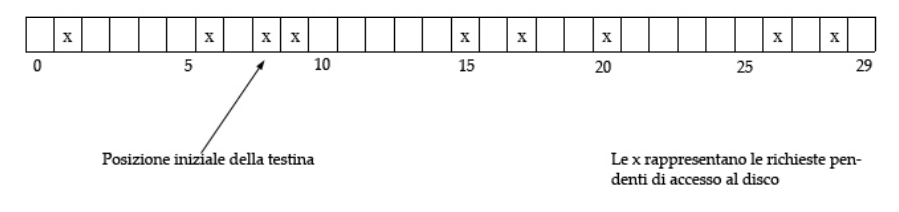
\includegraphics[width=0.9\textwidth]{scherm.png}
\end{figure}
\vskip 0.5cm
\textbf{Soluzione}\\
\vskip 0.5cm
(Teoria : I moderni sistemi operativi,da pag 296, paragrafo 5.4.3. Gli algoritmi di schedulazione del braccio del disco.)\\

\textbf{Algoritmo SSF} (Shortest Seek First): risolte per prima le richieste più vicine alla posizione attuale della testina. La posizione successiva k è stabilita dalla
formula seguente:
\[ \DeclareMathOperator{\argmin}{arg\,min}_k|(P-P_{k})| \]
\textbf{Algoritmo dell’ascensore:} risolte tutte le richieste in una direzione (salita, ad esempio), poi risolte quelle nell’altra direzione.\\
Garantisce la fairness del sistema, rendendo impossibile la starvation.\\

\textbf{Algoritmo SSF soluzione:}
\vskip 0.4cm

\begin{tabular}{|p{0.1\textwidth}|p{0.1\textwidth}|p{0.1\textwidth}|p{0.1\textwidth}|p{0.1\textwidth}|p{0.1\textwidth}|p{0.1\textwidth}|p{0.1\textwidth}|p{0.1\textwidth}|}

\hline
       &  &  &  &  &  &  &  &          \\
\hline
8     & 9 & 6 & 1 & 15 & 17 & 20 & 26 & 28      \\

\hline
\end{tabular}

\vskip 0.8cm
\textbf{Algoritmo dell’ascensore soluzione:}
\vskip 0.4cm

\begin{tabular}{|p{0.1\textwidth}|p{0.1\textwidth}|p{0.1\textwidth}|p{0.1\textwidth}|p{0.1\textwidth}|p{0.1\textwidth}|p{0.1\textwidth}|p{0.1\textwidth}|p{0.1\textwidth}|}

\hline
       &  &  &  &  &  &  &  &          \\
\hline
8     & 9 & 15 & 17 & 20 & 26 & 28 & 6 & 1      \\

\hline
\end{tabular}

\vskip 0.8cm

\end{document}